% Author: David Paulino
% Date: 2023-03-03
% Description: LaTeX Template


\documentclass[12pt]{article}

% Document en français
\usepackage[french]{babel}

\usepackage[utf8]{inputenc}
\usepackage[T1]{fontenc}
\usepackage{graphicx}
\usepackage{amsmath}
\usepackage{amssymb}
\usepackage{amsthm}
\usepackage{amsfonts}
\usepackage{amscd}
\usepackage{amstext}

\usepackage{hyperref}
\usepackage{xcolor}
\usepackage{fancyhdr}
\usepackage{setspace}
\usepackage{float}
\usepackage{subfig}
\usepackage{caption}
\usepackage{listings}
\usepackage{tikz}
\usepackage{pgfplots}
\usepackage{pgfplotstable}
\usepackage{pgf}

% Add references in table of contents
\usepackage[nottoc]{tocbibind}

% Set author and place
\newcommand{\DP}{David Paulino}
\newcommand{\place}{Genève}
\newcommand{\fulltitle}{Analyse et optimisation de l'expected goal: application au machine learning}
\newcommand{\shorttitle}{Analyse et optimisation de l'expected goal}

% Title
\title{Title}
\author{\DP}
\date{\today}

% Header
\pagestyle{fancy}
\fancyhf{}
\renewcommand{\headrulewidth}{0pt}
\lhead{\DP}
\rhead{\shorttitle}

% Footers
\lfoot{Page \thepage}
\rfoot{\today}

% Document
\begin{document}

% Title page
\begin{titlepage}

    \begin{figure}[h]
        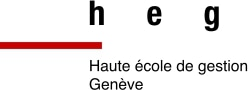
\includegraphics[width=0.3\textwidth]{img/logo_heg-ge.jpg}
    \end{figure}

    \vspace*{0.5cm}

    \begin{center}

        \begingroup \linespread{1,75} \selectfont
        {\Large \fulltitle}\\[0,75cm]
        \endgroup


        % Make a vertical space

        \vspace{1.5cm}

        \textsc{\large Travail de Bachelor HES réalisé en vue de \newline l’obtention du Bachelor par :}\\[0,50cm]

        \begingroup \linespread{1,75} \selectfont
        \textsc{\large \DP}\\[0,50cm]
        \endgroup


        \vspace{1cm}


        \textsc{\large Conseillers au travail de Bachelor : }

        \begingroup \linespread{1,75} \selectfont
        \textsc{\large Alexandros KALOUSIS}\\[0.1cm]
        \textsc{\large Nils SCHÄTTI}\\[1cm]
        \endgroup


        \begingroup \linespread{1,75} \selectfont
        \textsc{\large \place, le \today}\\[0,25cm]

        {\large Haute école de Gestion de Genève (HEG-GE)}\\[0,25cm]

        {\large Filière Informatique de gestion}\\[0,25cm]
        \endgroup



        \begin{figure}[h]
            \vspace*{1cm}
            \hspace*{12cm}
\includegraphics[width=0.25\textwidth]{img/logo_hes-so.jpg}
        \end{figure}

    \end{center}



    \vfill
\end{titlepage}




\newpage

% Table of contents
\tableofcontents
\newpage

% Content
\section{Introduction}

% Citation avec Zotero et BibLaTeX
\subsection{Introduction à la problématique}
\noindent La problématique de ce travail est de pouvoir analyser et optimiser l'expected goal.
\newline
Il est tout d'abord important d'introduire ce qu'est l'expected goal. L'expected goal\footnote{Très souvent réduit par xG} est une métrique qui permet de déterminer la probabilité qu'un tir soit transformé en but selon les données de ce tir \cite{XGExplainedFBrefa}. Un tir qui a un xG de 0.4 a une probabilité de 40\% d'être transformé en but. Un tir avec un xG à 1 est la plus grande valeur possible et aurait donc 100\% de chance d'être transformé en but. \footnote{Il est important d'indiquer qu'il est très rare qu'un xG d'un tir soit égal à 1 mais il va généralement sans rapprocher fortement selon ses paramètres.} \cite{pettyWhatExpectedGoals2018a}
\newline
La problématique m'a semblé cohérente par rapport à ma personnalité puisque je suis passionné par le football et que j'ai toujours été intéressé par les statistiques et les données. J'ai donc décidé de m'intéresser à l'expected goal et de voir comment on pouvait l'optimiser.
\subsection{Intérêt de la problématique}
\noindent Cette problématique est très intéressante puisque c'est une donnée qui est dernièrement très populaire dans le monde du football. Elle donne plus d'informations sur le match que les autres statistiques d'un matchs (possession, nombre de passes, nombre de tirs cadrés, nombre de buts, etc.). Par exemple en ce qui concerne la possession, une équipe peut avoir la possession du ballon pendant 70\% du match mais ne pas marquer de buts, ni même être dangereuse avec le ballon. Le nombre de tirs cadrés, s'ils sont effectuées tous à l'extérieur de la surface de réparation, ne sont pas forcément dangereux. L'expected goal permet de donner une valeur à chaque tir et de déterminer si un tir a une chance d'être transformé en but.
\newline \newline
Ensuite, certaines personnes utilisent cette métrique pour leurs paris sportifs. Ils observent la métrique lors des derniers matchs et la compare avec le score réel du match. Si la différence est grande, cela peut permettre de constater un manque de réalisme ou un sur-régime d'une des deux équipes. \cite{tennerelBienUtiliserExpected2022a}
\newline \newline
D'autres personnes utilisent cette donnée pour analyser les performances de leurs joueurs et de leurs équipes. Par exemple, la comparaison des xG et du nombre de buts marqués d'un joueur sur une période donnée peut permettre de déterminer la dangerosité et la capacité d'un buteur à terminer des actions. \cite{pettyWhatExpectedGoals2018a}
Les xG peuvent aussi être utilisés pour analyser les performances d'une équipe dans des situations bien précises. Une équipe qui possède un haut xG sur des contre-attaques montre qu'elle est très dangereuse sur ce type de situation. \cite{XGExplainedFBrefa}

\subsection{Questions que l'on souhaite répondre dans ce travail}
\noindent Il y a plusieurs questions qui peuvent se poser dans ce travail. Je vais donc les lister.
\begin{itemize}
    \item Comment est calculé l'expected goal ?
    \item Quels sont les paramètres qui influencent le plus l'expected goal ?
    \item Quel est le meilleur modèle pour prédire l'expected goal ?
    \item Quels sont les variables qui peuvent être ajoutée pour améliorer le résultat de la prédiction ?
    \item Quel est le meilleur modèle pour prédire l'expected goal en utilisant les variables ajoutées ?
\end{itemize}

\subsection{Intérêt de ces questions}
\noindent Le but de ces questions est de comprendre comment implémenter un modèle qui permet de prédire l'expected goal. Grâce à cela, on pourra ensuite connaître quels sont les variables obligatoires pour implémenter un tel modèle et quels sont les paramètres qui influencent le plus l'expected goal. Ensuite, on pourra voir quel est le meilleur modèle pour prédire l'expected goal et quels sont les variables qui peuvent être ajoutées pour améliorer le résultat de la prédiction. Enfin, on pourra voir quel est le meilleur modèle pour prédire l'expected goal en utilisant les variables ajoutées.
\section{Synthèse des travaux existants}
\label{sec:synthese}
% Application concrètes de mon travail ou alors applications déjà concrète de la problématique?
\noindent Parmi les travaux existants, il y a le travail de David Sumpter \cite{sumpterFittingXGModel} qui permet de comprendre comment implémenter un modèle d'expected goal. Ce travail va être une bonne base pour implémenter le premier modèle.
\newline
\noindent Ensuite, le travail nommé "Expected goals in soccer:explaining match results using predictive analytics" de Eggels \cite{eggelsExpectedGoalsSoccer2016} est un travail très détaillé qui permet d'avoir des pistes d'améliorations et qui explique bien les différentes étapes pour implémenter un modèle d'expected goal. Ce travail va être très utile pour permette d'apporter des améliorations au modèle.

\section{Dataset}

\subsection{Présentation du dataset}

\noindent Comme indiqué dans le section \ref{sec:synthese}, le travail de David Sumpter \cite{sumpterFittingXGModel} va être utilisé comme base pour implémenter le premier modèle. Il utilise un dataset qui contient les données de Wyscout. Wyscout est une entreprise qui fournit des données sur le football. Elle fournit des données sur les matchs, les joueurs, les équipes, les compétitions, etc. Il n'a pas été possible pour moi d'accéder au données directement par Wyscout. J'ai donc utilisé un dataset public qui est un sample du dataset de Wyscout. \cite{pappalardoPublicDataSet2019}
\newline
\noindent Cette source permet d'avoir l'information des événements lors d'un match de foot, comme par exemple les passes, les tirs, les fautes, etc. Cela permet d'avoir les informations nécessaires pour calculer l'expected goal. Un autre avantage de ce dataset est qu'il est déjà nettoyé et qu'il est facilement utilisable. Il est aussi très complet puisqu'il contient des données sur les matchs de 5 championnats européens (Angleterre, Espagne, Italie, Allemagne et France) de la saison 2017-2018. Il contient aussi des données sur les matchs de la coupe du monde 2018 et de l'Euro 2016.

% Description de chaque attribut dans le dataset event

% Description de chaque attribut dans le dataset players

% Bibliography
\bibliographystyle{plain}
\bibliography{bibliography}

\end{document}